% DOCUMENT CLASS %
\documentclass{article}

% PACKAGES%
\usepackage{amsfonts}   % For a basic mathfont (many will be replaced by stix)
\usepackage{amsmath}    % For basic math symbols
\usepackage{bbm}        % For \mathbbm (better version of \mathbb)
\usepackage{mathrsfs}   % For \mathscr
\usepackage{hyperref}   % For footnotes
\usepackage{csquotes}   % For \textquote{}
\usepackage{IEEEtrantools}  % For better alignments
\usepackage{tikz}   % For a macro
\usepackage{listings} % For code
\usepackage{xcolor}   % For ... code
\usepackage[utf8]{inputenc}  % Erlaubt es, Umlaute etc. zu verwenden (Datei muss UTF-8 Kodierung haben)
\usepackage[ngermanb]{babel} % Deutsche Übersetzung und Silbentrennung (Neue Rechtschreibung)

\usepackage{enumitem}
\setlist[itemize]{noitemsep}

\usepackage{fontspec}
\usepackage{unicode-math}

% FONT CONFIGURATION %
\setmainfont{Crimson Text}[
  BoldFont={Crimson Text Bold},
  SmallCapsFont={Times Small Caps & Old Style Fi},
  Ligatures={TeX,Common}
]
\setmathfont{Latin Modern Math}[Scale=MatchUppercase, FakeBold={2}]

% SETS %
\newcommand*{\R}{\mathbbm R}    % Set of real numbers
\newcommand*{\N}{\mathbbm N}    % Set of natural numbers (beginning at 0)
\newcommand*{\Z}{\mathbbm Z}    % Set of integers
\newcommand*{\Q}{\mathbbm Q}    % Set of rational numbers
\newcommand*{\pro}{\mathcal P}  % Power set of a set
\newcommand*{\Co}{\mathcal C^1}     % Set of R^n -> R^d functions that are fully partially differenciable and continuous
\newcommand*{\Ct}{\mathcal C^2}     % Set of R^n -> R functions that are C^1 functions and whose gradient is C^1 function
\newcommand*{\SetP}{\textup{P}}
\newcommand*{\SetNP}{\textup{NP}}
\newcommand*{\SetSAT}{\textup{SAT}}
\newcommand*{\SetClique}{\textup{Clique}}
\newcommand*{\SetKClique}{k\smi\textup{Clique}}
\newcommand*{\SetKColor}{k\smi\textup{Color}}


% OPERATIONS ON FUNCTIONS %
\newcommand*{\ddx}{\frac{\text d}{\text dx}}    % Derivative of a function
\newcommand*{\grad}{\text{grad}}    % Gradient of a function
\newcommand*{\J}{\textbf{J}}        % Jacobi-matrix of a function
\newcommand*{\He}{\textbf{H}}       % Hesse-matrix of a function
\newcommand*{\LMAX}{\text{\scshape Lmax}}   % Set of maxima of a function
\newcommand*{\LMIN}{\text{\scshape Lmin}}   % Set of minima of a function
\newcommand*{\img}{\text{img}}      % Image of a function
\newcommand*{\dom}{\text{dom}}      % Domain of a function

% DISTRIBUTIONS %
\newcommand*{\Unif}{\text{Unif}}    % Uniform distribution (discrete or continous)
\newcommand*{\Ber}{\text{Ber}}  % Bernoulli distribution
\newcommand*{\Bin}{\text{Bin}}  % Binomial distribution
\newcommand*{\Exp}{\text{Exp}}  % Exponential distribution
\newcommand*{\Geo}{\text{Geo}}  % Geometric distribution
\newcommand*{\Pois}{\text{Pois}}    % Poisson distribution
\newcommand*{\Norm}{\mathcal{N}}    % Normal distribution
\newcommand*{\D}{\mathcal{D}}   % Some random distribution

% BASIC PROBABILISTIC STUFF %
\newcommand*{\E}{\mathcal E}    % Some space of events
\newcommand*{\Pro}{\mathbbm P}  % Probability function of an event
\newcommand*{\Od}{\text{Od}}    % Odds of an event

% OPERATIONS ON DISTRIBUTIONS OR RANDOM VALUES %
\newcommand*{\supp}{\text{supp}}    % Support of a random variable
\newcommand*{\Ew}{\mathbbm E}   % Expected value
\newcommand*{\Var}{\text{Var}}  % Variance
\newcommand*{\Cov}{\text{Cov}}  % Covariance of two random variables
\newcommand*{\B}{\mathbbm B}    % Bias of a point estimation

% MACROS %
\newcommand{\subsubsubsection}[2]{\textsc{\underbar{#1}} \\#2\\\\}  % Macro for title in ALLCAPS, ends with two newlines
\newcommand*{\todo}{\textit{\dots TODO \dots}}  % Macro for ... todo ...
\newcommand*{\QDp}{{:}\text{ }} % Macro for ": " so that when writing something like "\forall x:" there is not a seperation between the '\forall' and the ':'
\newcommand*{\puffer}{\text{ }\text{ }\text{ }\text{ }} % Macro for a lazy aligment 1
\newcommand*{\gedanke}{\textbf{-- }}    % Macro for a long minus followed by text
\newcommand*{\smi}{\text{-}}        % Macro for a small minus ('-')
\newcommand*{\gap}{\text{ }}    % Macro for a lazy aligment 2
\newcommand*{\qed}{\null\nobreak\hfill\ensuremath{\square}} % Macro for a QED-Box
% for a funny ¯\_(ツ)_/¯-Emoji
\newcommand{\shrug}[1][]{%
    \begin{tikzpicture}[baseline,x=0.8\ht\strutbox,y=0.8\ht\strutbox,line width=0.125ex,#1]
    \def\arm{(-2.5,0.95) to (-2,0.95) (-1.9,1) to (-1.5,0) (-1.35,0) to (-0.8,0)};
    \draw \arm;
    \draw[xscale=-1] \arm;
    \def\headpart{(0.6,0) arc[start angle=-40, end angle=40,x radius=0.6,y radius=0.8]};
    \draw \headpart;
    \draw[xscale=-1] \headpart;
    \def\eye{(-0.075,0.15) .. controls (0.02,0) .. (0.075,-0.15)};
    \draw[shift={(-0.3,0.8)}] \eye;
    \draw[shift={(0,0.85)}] \eye;
    % draw mouth
    \draw (-0.1,0.2) to [out=15,in=-100] (0.4,0.95); 
    \end{tikzpicture}
}

% ADJUSTMENTS OF PAPER %                                                                                                                                                                                                                
\setlength{\hoffset}{-1.5cm}
\setlength{\voffset}{-2.5cm}
\setlength{\textheight}{24cm} % DIN A4 ~ 30cm
\setlength{\textwidth}{15cm}  % DIN A4 = 21cm, 18 suffice.

% Für deutsche Dokumente
\renewcommand{\contentsname}{Inhalt}
\renewcommand{\partname}{Teil}

\lstdefinestyle{mystyle}{
    basicstyle=\ttfamily\footnotesize,  % the size of the fonts that are used for the code
    breakatwhitespace=false,            % sets if automatic breaks should only happen at whitespace
    breaklines=true,                    % sets automatic line breaking
    frame=leftline,
    keepspaces=true,                    % keeps spaces in text, useful for keeping indentation of code (possibly needs columns=flexible)
    numbers=left,                       % where to put the line-numbers; possible values are (none, left, right)
    numbersep=5pt,                      % how far the line-numbers are from the code
    showspaces=false,                   % show spaces everywhere adding particular underscores; it overrides 'showstringspaces'
    showstringspaces=false,             % underline spaces within strings only
    showtabs=false,                     % show tabs within strings adding particular underscores
    tabsize=2,                          % sets default tabsize to 4 spaces
    commentstyle=\sffamily\itshape,
    emph={*, do, od, for, if, fi, then, else, to, def, in, forall, exists, while}, 
    emphstyle={\sffamily\bfseries},
    keywordstyle={\sffamily\bfseries},   % emphasis style for the keywords,
    texcl=true
}

\lstset{style=mystyle}



\usepackage{booktabs}

\newcommand{\nr}{5}
\title{Data Science Assignment \nr}
\author{Nike Marie Pulow -- Henri Paul Heyden \\ \small stu239549 -- stu240825}
\date{}

\begin{document}
    \maketitle
    \section{R-Tree}
    The following is an illustrated computation of the 7 insertions and needed splits. \\
    The first 2 insertions were not included since they are trivial.
    \begin{center}
        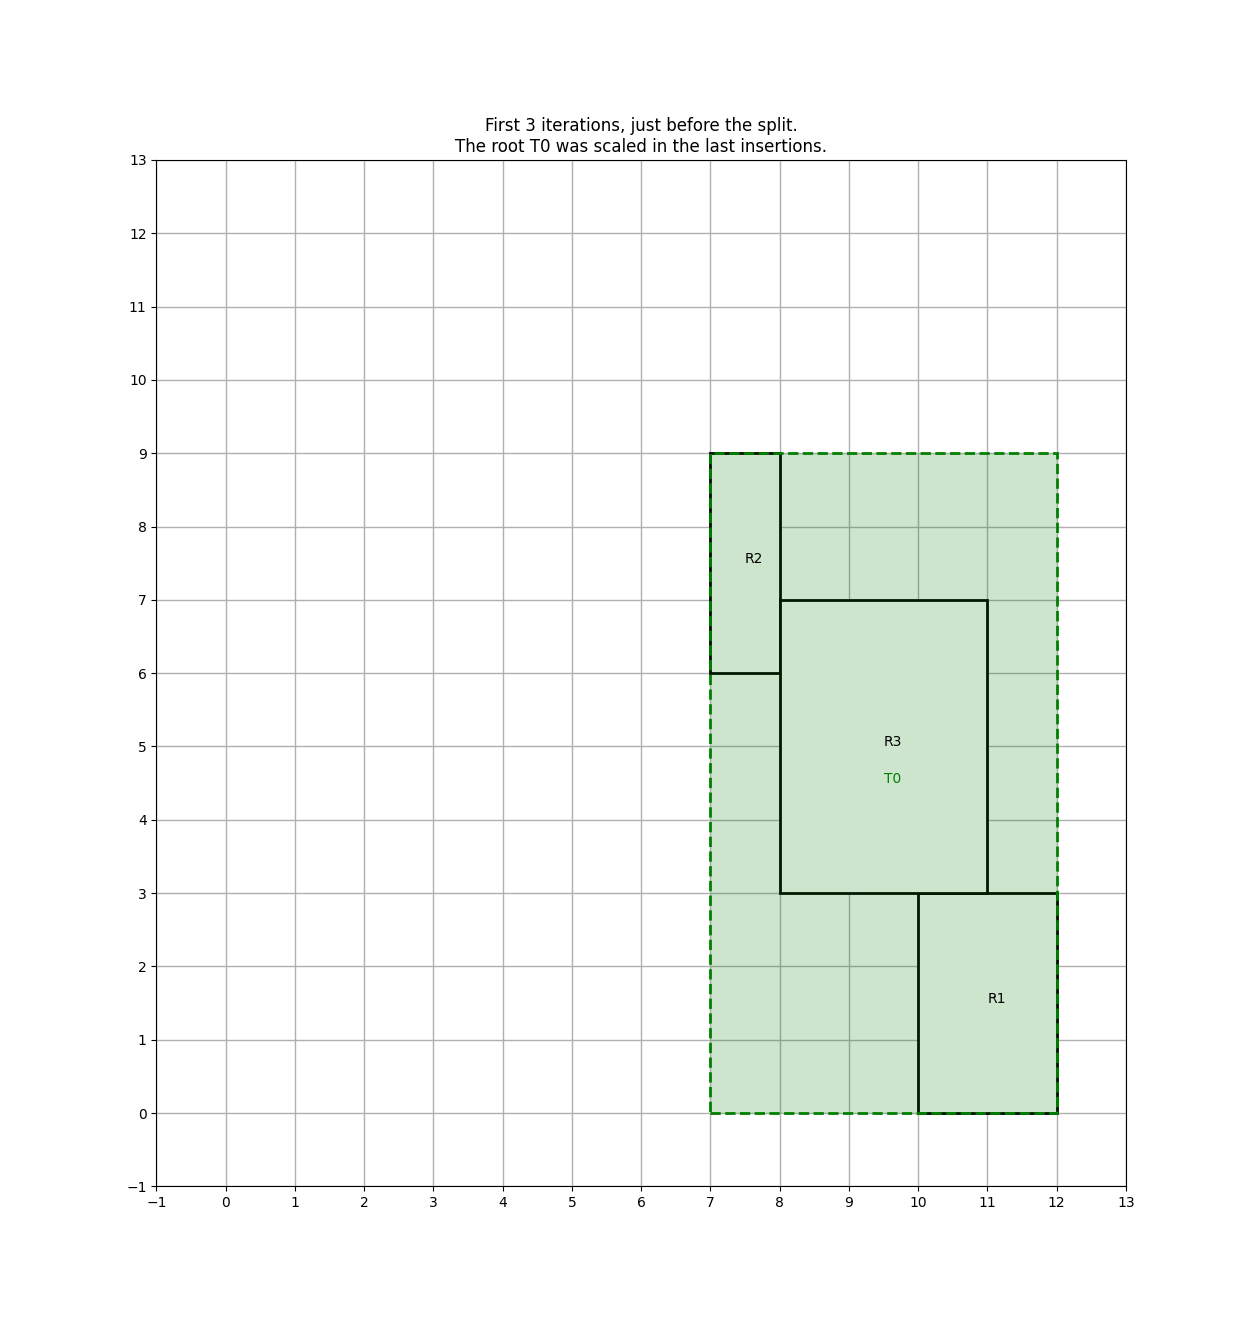
\includegraphics[scale=0.5]{./A1 figs/iter3.png}
        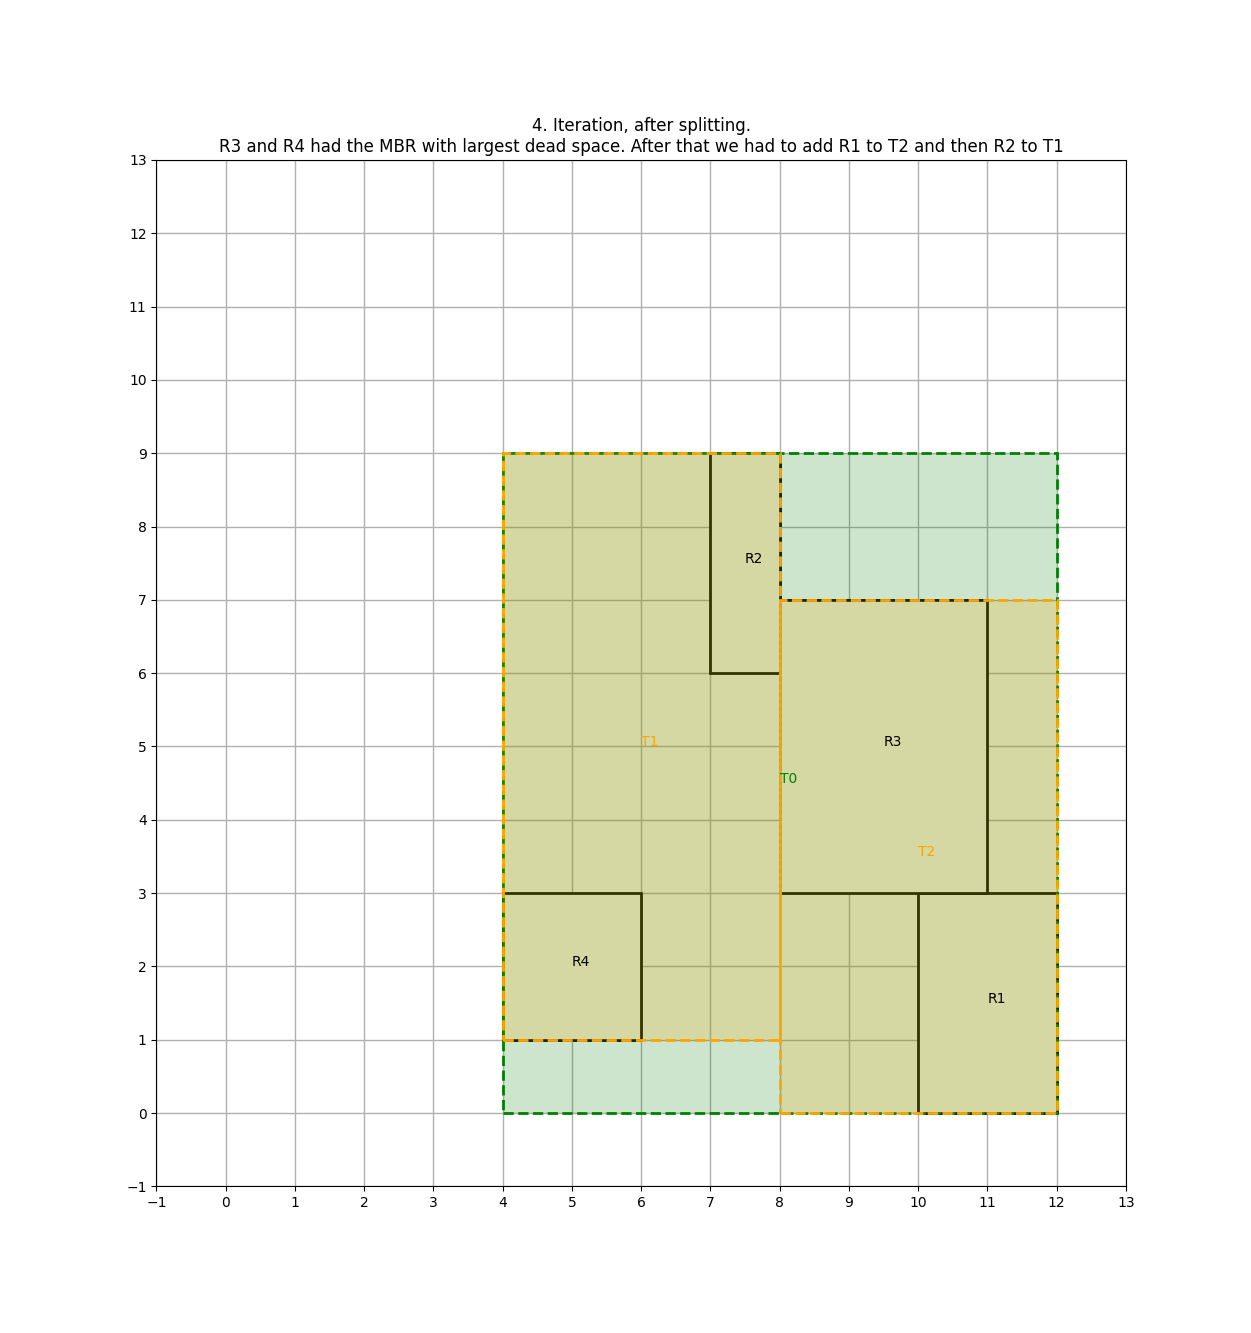
\includegraphics[scale=0.5]{./A1 figs/iter4.png}
        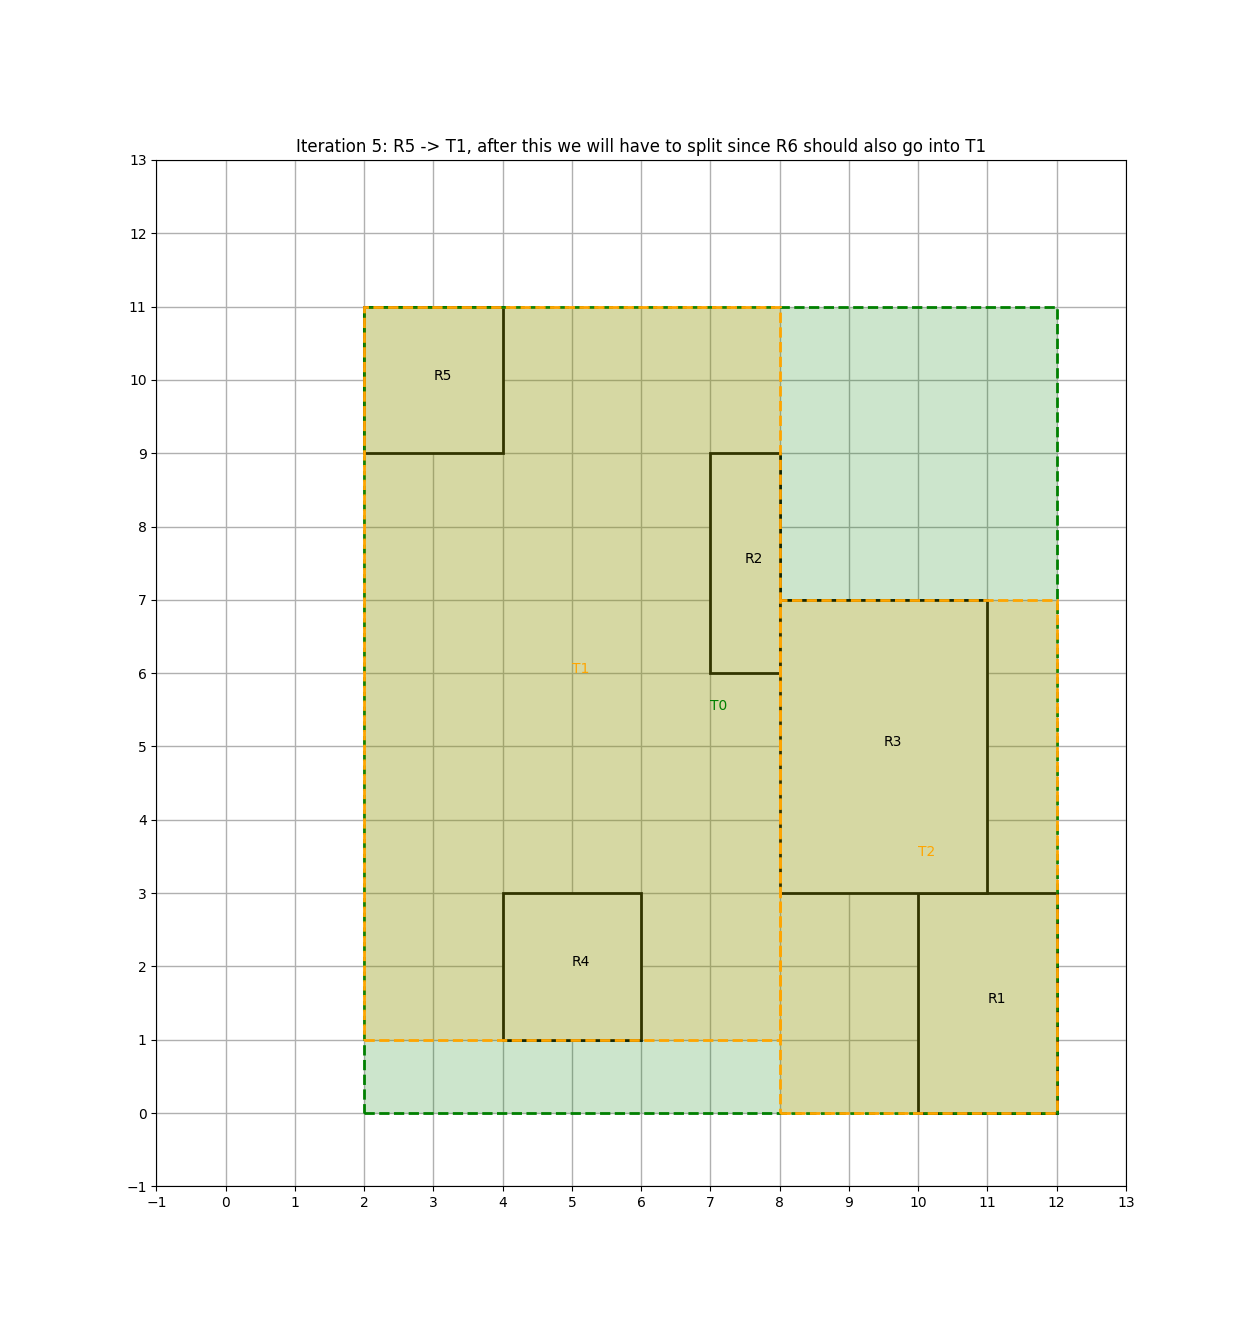
\includegraphics[scale=0.5]{./A1 figs/iter5.png}
        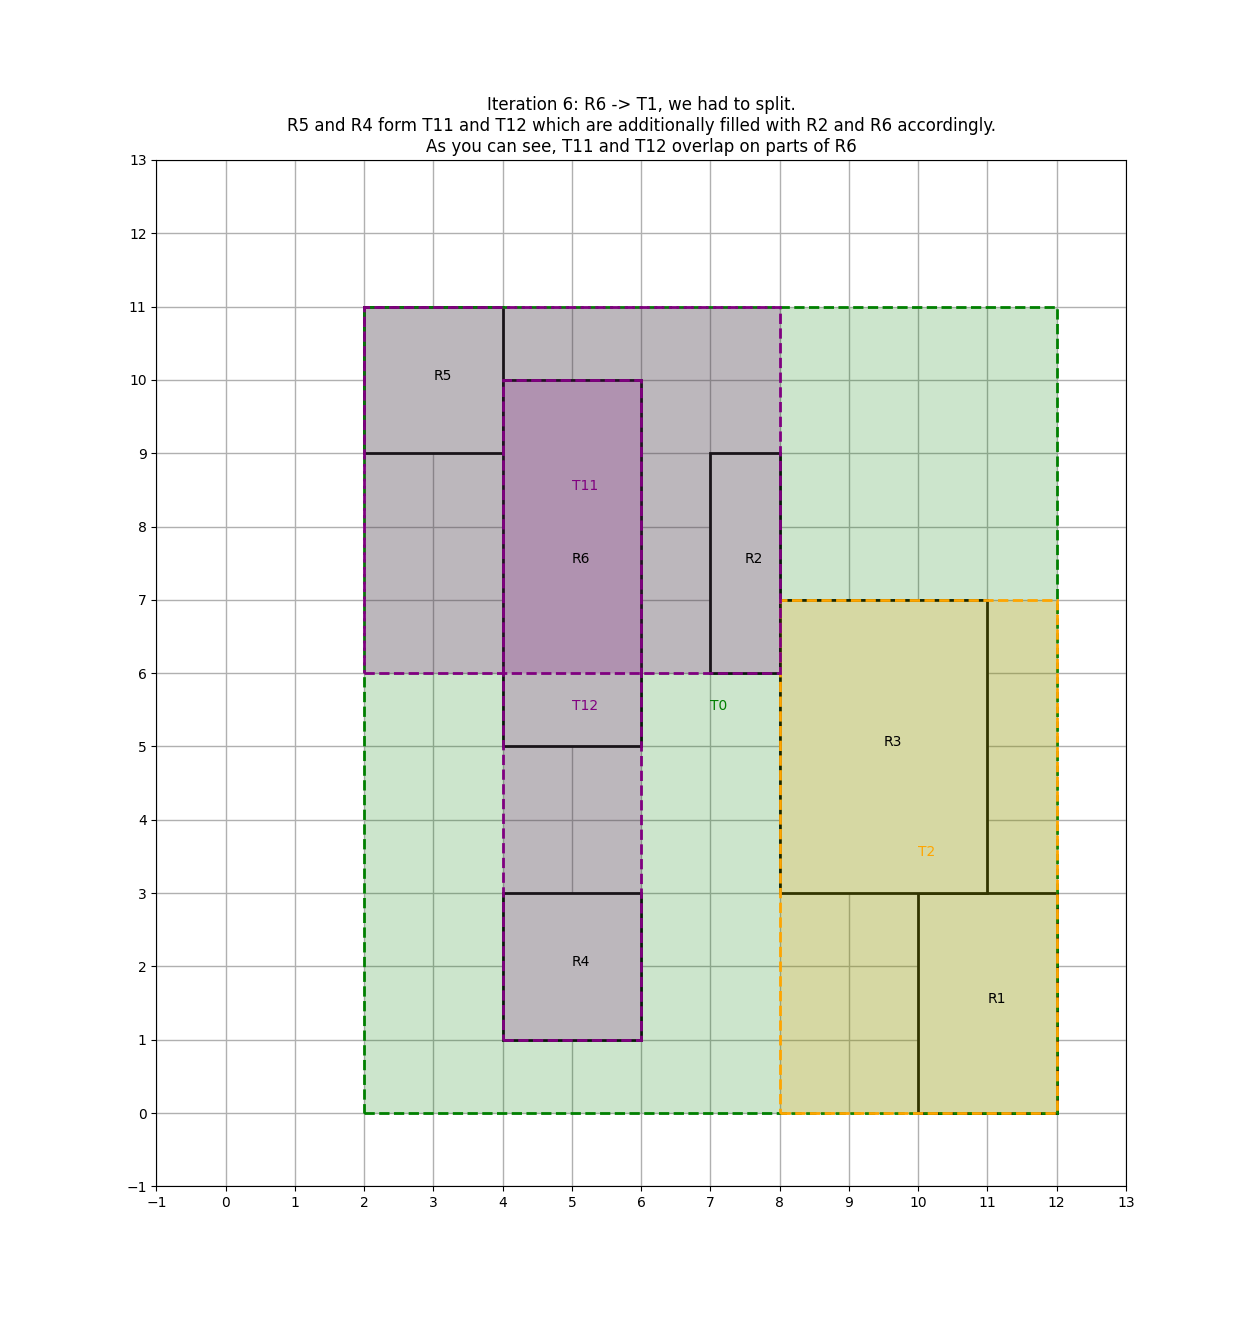
\includegraphics[scale=0.5]{./A1 figs/iter6.png}
        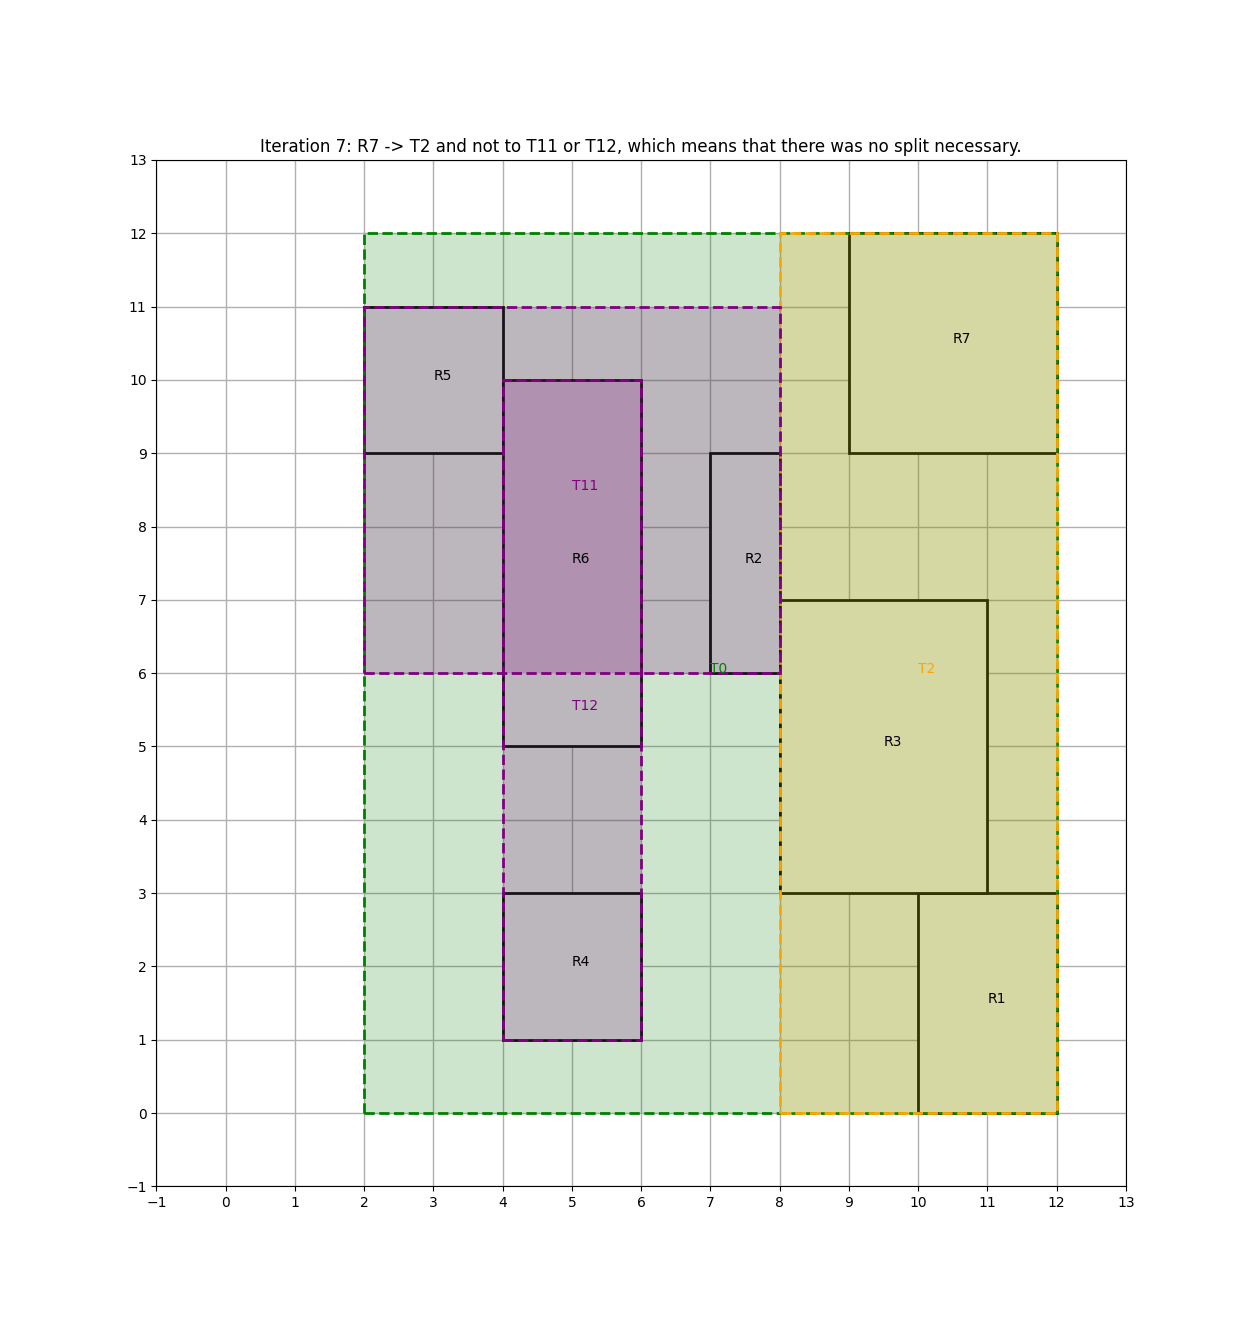
\includegraphics[scale=0.5]{./A1 figs/iter7.png}
    \end{center}
\pagebreak
    \section{\(k\)NN-Index-APL}
    \textbf{1:} \(q=(9,9)\), \(k=3\)\\
    \begin{tabular}{l | l | l | l}
        Iteration   & APL               & \textit{result}                                               & \textit{pruningdist} \\
        \toprule
        1.          & [(0,R1), (0,R2)]   & [(\(\infty, null\)), (\(\infty, null\)), (\(\infty, null\))]  & \(\infty\) \\
        2.          & [(0,R2), (0,A), (0,B)] & [(\(\infty, null\)), (\(\infty, null\)), (\(\infty, null\))] & \(\infty\) \\
        3.          & [(0,A), (0,B), (4,R21), (4,R22)] & [(\(\infty, null\)), (\(\infty, null\)), (\(\infty, null\))] & \(\infty\) \\
        4.          & [(0,B), (4,R21), (4,R22)] & [(3,A), (\(\infty, null\)), (\(\infty, null\))] & \(\infty\) \\
        5.          & [(4,R21), (4,R22)] & [(3,A), (13,B), (\(\infty, null\))] & \(\infty\) \\
        6.          & [(4,R22), (6,C), (6,D)] & [(3,A), (13,B), (\(\infty, null\))] & \(\infty\) \\
        7.          & [(4,E), (4,F), (6,C), (6,C)] & [(3,A), (13,B), (\(\infty, null\))] & \(\infty\) \\
        8.          & [(4,F), (6,C), (6,D)] & [(3,A), (6,E), (13,B)] & \(13\) \\
        9.          & [(6,C), (6,D)] & [(3,A), (6,E), (6,F)] & \(6\) \\
        10.         & [(6,D)] & [(3,A), (6,E), (6,F)] & \(6\) \\
        11.         & [] & [(3,A), (6,E), (6,F)] & \(6\) \\

    \end{tabular}
    \\
    \\
    \textbf{2:} \(q=(4,6)\), \(k=2\)\\
    \begin{tabular}{l|l|l|l}
        Iteration   & APL               & \textit{result}                                               & \textit{pruningdist} \\
        \toprule
        1. & [(0,R1), (0,R2)] & [(\(\infty, null\)), (\(\infty, null\))] & \(\infty\) \\
        2. & [(0,R2), (2,A), (2,B)] & [(\(\infty, null\)), (\(\infty, null\))] & \(\infty\) \\
        3. & [(1,R21), (1,R22), (2,A), (2,B)] & [(\(\infty, null\)), (\(\infty, null\))] & \(\infty\) \\
        4. & [(1,R22), (2,A), (2,B), (4,C), (4,D)] & [(\(\infty, null\)), (\(\infty, null\))] & \(\infty\) \\
        5. & [(2,A), (2,B), (2,E), (2,F), (4,C), (4,D)] & [(\(\infty, null\)), (\(\infty, null\))] & \(\infty\) \\
        6. & [(2,B), (2,E), (2,F), (4,C), (4,D)] & [(6,A), (\(\infty, null\))] & \(\infty\) \\
        7. & [(2,E), (2,F), (4,C), (4,D)] & [(6,A), (14,B)] & \(14\) \\
        8. & [(2,F), (4,C), (4,D)] & [(2,E), (6,A)] & \(6\) \\
        9. & [(4,C), (4,D)] & [(2,E), (2,F)] & \(2\) \\
    \end{tabular}
    \\
    \\
    \textbf{3:} \(q=(7,5)\), \(k=2\)\\
    \begin{tabular}{l|l|l|l}
        Iteration   & APL               & \textit{result}                                               & \textit{pruningdist} \\
        \toprule
        1. & [(0,R1), (0,R2)] & [(\(\infty, null\)), (\(\infty, null\))] & \(\infty\) \\
        2. & [(0,R2), (3,A), (3,B)] & [(\(\infty, null\)), (\(\infty, null\))] & \(\infty\) \\
        3. & [(0,R21), (0,R22), (3,A), (3,B)] & [(\(\infty, null\)), (\(\infty, null\))] & \(\infty\) \\
        4. & [(0,R22), (2,C), (2,D), (3,A), (3,B)] & [(\(\infty, null\)), (\(\infty, null\))] & \(\infty\) \\
        5. & [(0,E), (0,F), (2,C), (2,D), (3,A), (3,B)] & [(\(\infty, null\)), (\(\infty, null\))] & \(\infty\) \\
        6. & [(0,F), (2,C), (2,D), (3,A), (3,B)] & [(2,E), (\(\infty, null\))] & \(\infty\) \\
        7. & [(2,C), (2,D), (3,A), (3,B)] & [(2,E), (2,F)] & 2 \\
        8. & [(2,D), (3,A), (3,B)] &  [(2,E), (2,F)] & 2 \\
        9. & [(3,A), (3,B)] & [(2,E), (2,F)] & 2 \\
    \end{tabular}
    \\
    \\
    \textbf{4: } TODO
\end{document}
